\documentclass[]{article}
\hyphenation{co-rres-pon-dien-tes te-ner E-ben-sper-ger de-pre-da-do-res dis-po-ni-ble be-ne-fi-cio-sa in-di-vi-dual so-cia-li-dad mos-tra-ron fuen-tes a-cep-ta-ble ta-ma-ño o-pues-ta mo-de-lo es-tu-dian-tes e-jer-ci-cios co-rres-pon-dien-te mo-di-fi-ca-dos mo-di-fi-car-lo ma-ni-pu-lar}
\usepackage{amssymb,amsmath}
\usepackage{ifxetex,ifluatex}
\ifxetex
  \usepackage{fontspec,xltxtra,xunicode}
  \defaultfontfeatures{Mapping=tex-text,Scale=MatchLowercase}
\else
  \ifluatex
    \usepackage{fontspec}
    \defaultfontfeatures{Mapping=tex-text,Scale=MatchLowercase}
  \else
    \usepackage[utf8]{inputenc}
  \fi
\fi
\usepackage{color}
\usepackage{fancyvrb}
\DefineShortVerb[commandchars=\\\{\}]{\|}
\DefineVerbatimEnvironment{Highlighting}{Verbatim}{commandchars=\\\{\}}
% Add ',fontsize=\small' for more characters per line
\newenvironment{Shaded}{}{}
\newcommand{\KeywordTok}[1]{\textcolor[rgb]{0.00,0.44,0.13}{\textbf{{#1}}}}
\newcommand{\DataTypeTok}[1]{\textcolor[rgb]{0.56,0.13,0.00}{{#1}}}
\newcommand{\DecValTok}[1]{\textcolor[rgb]{0.25,0.63,0.44}{{#1}}}
\newcommand{\BaseNTok}[1]{\textcolor[rgb]{0.25,0.63,0.44}{{#1}}}
\newcommand{\FloatTok}[1]{\textcolor[rgb]{0.25,0.63,0.44}{{#1}}}
\newcommand{\CharTok}[1]{\textcolor[rgb]{0.25,0.44,0.63}{{#1}}}
\newcommand{\StringTok}[1]{\textcolor[rgb]{0.25,0.44,0.63}{{#1}}}
\newcommand{\CommentTok}[1]{\textcolor[rgb]{0.38,0.63,0.69}{\textit{{#1}}}}
\newcommand{\OtherTok}[1]{\textcolor[rgb]{0.00,0.44,0.13}{{#1}}}
\newcommand{\AlertTok}[1]{\textcolor[rgb]{1.00,0.00,0.00}{\textbf{{#1}}}}
\newcommand{\FunctionTok}[1]{\textcolor[rgb]{0.02,0.16,0.49}{{#1}}}
\newcommand{\RegionMarkerTok}[1]{{#1}}
\newcommand{\ErrorTok}[1]{\textcolor[rgb]{1.00,0.00,0.00}{\textbf{{#1}}}}
\newcommand{\NormalTok}[1]{{#1}}
% Redefine labelwidth for lists; otherwise, the enumerate package will cause
% markers to extend beyond the left margin.
\makeatletter\AtBeginDocument{%
  \renewcommand{\@listi}
    {\setlength{\labelwidth}{4em}}
}\makeatother
\usepackage{enumerate}
\usepackage{graphicx}
% We will generate all images so they have a width \maxwidth. This means
% that they will get their normal width if they fit onto the page, but
% are scaled down if they would overflow the margins.
\makeatletter
\def\maxwidth{\ifdim\Gin@nat@width>\linewidth\linewidth
\else\Gin@nat@width\fi}
\makeatother
\let\Oldincludegraphics\includegraphics
\renewcommand{\includegraphics}[1]{\Oldincludegraphics[width=\maxwidth]{#1}}
\ifxetex
  \usepackage[setpagesize=false, % page size defined by xetex
              unicode=false, % unicode breaks when used with xetex
              xetex,
              colorlinks=true,
              linkcolor=blue]{hyperref}
\else
  \usepackage[unicode=true,
              colorlinks=true,
              linkcolor=blue]{hyperref}
\fi
\hypersetup{breaklinks=true, pdfborder={0 0 0}}
\setlength{\parindent}{0pt}
\setlength{\parskip}{6pt plus 2pt minus 1pt}
\setlength{\emergencystretch}{3em}  % prevent overfull lines
\setcounter{secnumdepth}{0}


\begin{document}

\section{Ejercicios de programación IV: Funciones}

\subsubsection{{[}IMSER 2012{]}}

\begin{center}\rule{3in}{0.4pt}\end{center}

\subsection{Archivos incluidos:}

El
\href{http://eva.universidad.edu.uy/file.php/1454/ejercicios\_de\_programacion/rep-1.zip}{archivo}
con los ejercicios del práctico debe bajarse y descomprimirse en disco
duro, creando la carpeta \textbf{\texttt{rep-2}} (nota: no debe dentro
de ningún disco, partición o carpeta protegida a la escritura, como
puede ser un disco duro externo de backup). Usted deberá abrir el
RStudio y seleccionar dicha carpeta como su directorio de trabajo con
\texttt{setwd} o en RStudio la combinación \textbf{Ctrl + Shift + K}. En
esta carpeta se encuentran algunos archivos que usted deberá modificar:

\begin{itemize}
\item
  \textbf{\texttt{triangulo.R}}
\item
  \textbf{\texttt{educacion.R}}
\item
  \textbf{\texttt{cambiaPares.R}}
\item
  \textbf{\texttt{radio.R}}
\item
  \textbf{\texttt{distancias.R}}
\end{itemize}
Adicionalmente los siguientes archivos son necesarios, pero \textbf{no
deben ser modificados} para que el método de calificación automático
funcione correctamente:

\begin{itemize}
\item
  \texttt{datos}
\item
  \texttt{evaluar}
\item
  \texttt{notas.csv}
\item
  \texttt{edu.data.rda}
\item
  \texttt{HandbookSpanish.pdf}
\item
  \texttt{INSTRUCCIONES.pdf}
\end{itemize}
\subsection{Mecanismo de corrección:}

Lo primero que debe hacer es cargar el archivo evaluar.R con la función
\texttt{source} y la codificación de caracteres ``UTF-8'' (lo cual
afecta a la función \texttt{evaluar} en particular), de la siguiente
manera:

\begin{Shaded}
\begin{Highlighting}[]
\KeywordTok{options}\NormalTok{(}\DataTypeTok{encoding =} \StringTok{"utf-8"}\NormalTok{)}
\KeywordTok{source}\NormalTok{(}\StringTok{"evaluar.R"}\NormalTok{)}
\end{Highlighting}
\end{Shaded}
Si usted ha ejecutado todos los pasos anteriores correctamente, la
siguiente frase debería verse en la consola:

\begin{verbatim}
Archivo de codigo fuente cargado correctamente
\end{verbatim}
En caso de que ocurra un error o se vea otro mensaje en la consola,
verifique que los archivos se descomprimieron correctamente y que usted
está trabajando en la carpeta correspondiente con el comando
\texttt{getwd()}.

Usted trabajará modificando los contenidos de dichos archivos con
RStudio (u otro programa de su preferencia) según las consignas que se
describen a continuación. Luego de terminar cada ejercicio y
\textbf{guardando el archivo} correspondiente en el disco duro, usted
podrá verificar rápidamente si su respuesta es correcta ejecutando el
comando:

\begin{Shaded}
\begin{Highlighting}[]
\KeywordTok{evaluar}\NormalTok{()}
\end{Highlighting}
\end{Shaded}
y además podrá en todo momento verificar su puntaje con la función
\texttt{verNotas()}. Tenga siempre en cuenta que, a \textbf{menos que
sea indicado} por la letra del ejercicio, las soluciones deben ser
genéricas y por lo tanto deben obtenerse con el código de los scripts en
lugar de ser valores fijos. Usualmente se utilizan valores generados de
forma aleatoria para las correcciones automáticas. Los objetos que son
evaluados en la corrección automática estarán indicados con un asterísco
en las instrucciones de cada script. Nótese además que en los archivos
\textbf{se indica claramente en dónde se inicia y dónde finaliza su
código} y que debe respetar esta organización para que la corrección de
los ejercicios funcione bien.

\subsubsection{Al finalizar}

Una vez terminados y guardados los archivos de los ejercicios del
repartido, usted deberá ejecutar \texttt{evaluar()} y seleccionar la
última opción (``Todos'') y luego subir el archivo ''datos'' (sin
extensión), incluido en la carpeta ''rep-1'', a la
\href{http://eva.universidad.edu.uy/mod/assignment/view.php?id=95125}{sección
de entregas} de la portada del curso en la plataforma EVA. Este archivo
se podrá reemplazar con uno más nuevo, en caso de que desee corregir
algún error; en caso de querer que el archivo sea corregido antes de la
fecha de entrega, puede cambiarle el nombre a ``datos-finalizado'', pero
en ese caso la nota no se cambiará de ahí en adelante.

\subsubsection{Código de Honor}

Si bien animamos a que los estudiantes trabajen en equipos y que haya un
intercambio fluido en los foros del curso, es fundamental que las
respuestas a los cuestionarios y ejercicios de programación sean fruto
del trabajo individual. En particular, consideramos importante que los
estudiantes no miren el código creado por sus compañeros ya que esto
supone un sabotaje a su propio proceso de aprendizaje. Como profesores
estamos comprometidos a pedir tareas para las cuales hayamos dado las
herramientas correctas y las explicaciones adecuadas como para que todos
puedan encontrar su propio camino para resolver los ejercicios.

\begin{center}\rule{3in}{0.4pt}\end{center}

\subsection{1. Triángulos, volumen II}

Script: triangulo.R

Si hacemos un poco de memoria recordaremos el ejercicio 1 del repartido
I. En el mismo tomábamos los catetos de un triángulo rectángulo y
escribíamos el código necesario para calcular el valor de la hipotenusa
y el área del mismo. Como recordaremos, el valor de la hipotenusa se
calcula como:

\[
hip = \sqrt{cat.op ^ 2 + cat.ad ^ 2}
\]

mientras que el área del triángulo es:

\[
A = \frac{cat.op \cdot cat.ad}{2}
\]

A partir de los valores de los catetos y de la hipotenusa es posible
calcular el valor de los restantes ángulos del triángulo, siendo el
ángulo adyacente

\[
\alpha_{ad} = arccos \left( \frac{cat.ad}{hip} \right)
\]

y el ángulo opuesto

\[
\alpha_{op} = arccos \left( \frac{cat.op}{hip} \right)
\]

En el presente ejercicio debemos escribir el código de una función
llamada \texttt{triangulo} que, a partir de los mismos datos de las
funciones \texttt{area} e \texttt{hipot} de aquella ocasión, o sea de
los catetos de un triángulo rectángulo, calcule la hipotenusa, el área y
los ángulos adyacente y opuesto del triángulo. La salida de la función
deberá ser una lista con los objetos denominados de la siguiente manera:
\texttt{hipotenusa}, \texttt{area}, \texttt{angulo.adyacente} y
\texttt{angulo.opuesto}, en ese orden. Los ángulos deberán estar
expresados en grados. En R, la salida de las funciones trigonométricas,
como \texttt{asin} y \texttt{acos} están expresadas en radianes, por lo
que se deberá hacer la transformación correspondiente, teniendo en
cuenta que $\pi$ radianes equivalen a $180^o$.

A modo de ejemplo, la salida deseada al evaluar esta función con el
cateto adyacente y el opuesto valiendo respectivamente 4 y 3, sería la
siguiente:

\begin{Shaded}
\begin{Highlighting}[]
\KeywordTok{triangulo}\NormalTok{(}\DecValTok{4}\NormalTok{, }\DecValTok{3}\NormalTok{)}
\NormalTok{$hipotenusa}
\NormalTok{[}\DecValTok{1}\NormalTok{] }\DecValTok{5}

\NormalTok{$area}
\NormalTok{[}\DecValTok{1}\NormalTok{] }\DecValTok{6}

\NormalTok{$angulo.adyacente}
\NormalTok{[}\DecValTok{1}\NormalTok{] }\FloatTok{36.8699}

\NormalTok{$angulo.opuesto}
\NormalTok{[}\DecValTok{1}\NormalTok{] }\FloatTok{53.1301}
\end{Highlighting}
\end{Shaded}
\begin{center}\rule{3in}{0.4pt}\end{center}

\subsection{2. Educación}

Script: educacion.R

La Organización de la Naciones Unidas (ONU) en el año 2011
\href{http://mdgs.un.org/unsd/mdg/Resources/Static/Products/Progress2011/11-31342\%20\%28S\%29\%20MDG\%20Report\%202011\_Book\%20LR.pdf}{presentó
un informe} basado en indicadores utilizados para medir y supervisar los
Objetivos de Desarrollo del Milenio (ODM).

\begin{quote}
``La Declaración del Milenio de las Naciones Unidas de 2000, basada en
las conferencias mundiales de las Naciones Unidas durante el decenio de
1990, representó un fuerte compromiso con el derecho al desarrollo, la
paz y la seguridad, la igualdad de género, la erradicación de las
numerosas dimensiones de la pobreza y el desarrollo humano sostenible.
En la Declaración, adoptada por 147 jefes de Estado y 189 Estados, se
incorporaban lo que ha llegado a conocerse con el nombre de `ocho
objetivos de desarrollo del milenio', incluidas 18 metas con plazos
cronológicos delimitados''
(\href{http://unstats.un.org/unsd/publication/seriesf/Seriesf\_95s.pdf}{Fuente}).

\end{quote}
Para este ejercicio se utilizarán tres de los indicadores que han sido
propuestos para cumplir con el objetivo 2 de los ODM
\href{http://www.undp.org/content/undp/es/home/mdgoverview/mdg\_goals/mdg2/}{Lograr
la enseñanza primaria universal}:

\begin{itemize}
\item
  Tasa Neta de Matriculación en la Enseñanza Primaria (TM).
\item
  Porcentaje de alumnos que comienzan el primer grado y llegan al quinto
  grado (PA).
\item
  Tasa de alfabetización de personas entre 15 y 24 años (TA).
\end{itemize}
Las tres variables están expresadas en porcentaje. El objetivo es
realizar un cálculo grueso del porcentaje de niños que completan la
educación primaria (PC) para ciertos paises, a partir de TA y PA, usando
la fórmula: $PC = (TM \cdot PA) / 100$. Finalmente se hará una regresión
entre la tasa de alfabetización y el porcentaje de conclusión de
primaria calculado.

El archivo ``edu.data.rda'' contiene una data.frame llamada
\texttt{edu.data} con datos de varios años para ciertos países, usando
las abreviaciones de arriba para cada indicador (importar a R con
\texttt{load} o los botones de RStudio). Los datos fueron extraidos de
la \href{http://mdgs.un.org/unsd/mdg/Data.aspx}{portada oficial} de la
ONU para los indicadores de los OMD.

\paragraph{Entradas:}

ud. deberá crear una función llamada \texttt{educación}, la cual deberá
aceptar los siguientes argumentos, en este orden (si quiere puede
asignar valores por defecto a uno o a varios de estos argumentos):

\begin{itemize}
\item
  \texttt{x}: data.frame con los datos de entrada (\texttt{edu.data}).
\item
  \texttt{tmcol}: columnas correspondientes al indicador TM (en números
  o nombres, debería ser irrelevante).
\item
  \texttt{pacol}: columnas correspondientes al indicador PA (en números
  o nombres, debería ser irrelevante).
\item
  \texttt{tacol}: columna correspondiente al indicador TA (en número o
  nombre, debería ser irrelevante).
\end{itemize}
\paragraph{Acciones:}

la función deberá realizar los siguiente pasos:

\begin{enumerate}[1.]
\item
  Calcular, por país/fila, el promedio de los valores de TM y de PA.
\item
  Calcular con estos el valor promedio de PC para cada país.
\item
  Agregar estos tres valores calculados como columnas a la data.frame de
  entrada (\texttt{x}).
\item
  Realizar una regresión lineal de TA en función de PC.
\item
  Devolver los valores calculados y los datos más importantes de la
  regresión.
\end{enumerate}
Nota: los cálculos de promedios deben hacerse dejando de lado los
valores \texttt{NA}.

\paragraph{Salida:}

\texttt{educacion} debe devolver un objeto de clase \texttt{list}, el
cual debe contener los siguientes objetos (y en el mismo orden):

\begin{itemize}
\item
  \texttt{coeficientes}: los coeficientes de la regresión de TA en
  función de PC.
\item
  \texttt{p.valor}: el p.valor de la regresión correspondiente a los
  coeficientes (ver salida de \texttt{summary} para obtenerlos).
\item
  \texttt{r2}: el coeficiente de determinación ($R^2$) de la regresión
  (el cual puede calcularse usando una fórmula o la función
  \texttt{summary}).
\item
  \texttt{datos}: data.frame con los datos originales más las columnas
  correspondientes a los promedios de TM, PA y PC, en ese orden.
\end{itemize}
Nota: la función \texttt{summary} además de imprimir en la consola datos
útiles de una regresión, también genera una \textbf{salida invisible}
(ver lección 5.3).

El siguiente es un ejemplo obtenido con los datos y una función
\texttt{educacion} completada (la figura incluida también se generó con
esta función, pero para la tarea es opcional):

\begin{Shaded}
\begin{Highlighting}[]
\KeywordTok{load}\NormalTok{(}\StringTok{"edu.data.rda"}\NormalTok{)}
\NormalTok{x <- }\KeywordTok{educacion}\NormalTok{(edu.data, }\DecValTok{1}\NormalTok{:}\DecValTok{5}\NormalTok{, }\DecValTok{6}\NormalTok{:}\DecValTok{10}\NormalTok{, }\DecValTok{11}\NormalTok{)}
\end{Highlighting}
\end{Shaded}
\begin{figure}[htbp]
\centering
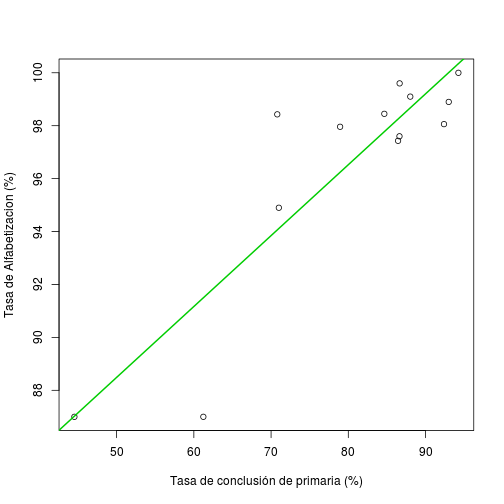
\includegraphics{figure/unnamed-chunk-5.png}
\caption{regresión de TA en función de PC (salida gráfica opcional de la
función educacion)}
\end{figure}

\begin{Shaded}
\begin{Highlighting}[]
\NormalTok{x$coeficientes}
\end{Highlighting}
\end{Shaded}
\begin{verbatim}
## (Intercept)          PC 
##     75.0948      0.2679 
\end{verbatim}
\begin{Shaded}
\begin{Highlighting}[]
\NormalTok{x$p.valor}
\end{Highlighting}
\end{Shaded}
\begin{verbatim}
## (Intercept)          PC 
##   2.329e-10   6.259e-05 
\end{verbatim}
\begin{Shaded}
\begin{Highlighting}[]
\NormalTok{x$r2}
\end{Highlighting}
\end{Shaded}
\begin{verbatim}
## [1] 0.7803
\end{verbatim}
\begin{center}\rule{3in}{0.4pt}\end{center}

\subsection{3. Funciones en problemas}

En este ejercicio se propone arreglar el código de algunas funciones
simples (y otra no tan simple). Para esto la idea es utilizar los
métodos y conceptos vertidos en la lección 5.4: \textbf{Depuración de
funciones}.

\subsubsection{3.a Cambiador de valores en subíndices pares\ldots{}}

Script: cambiaPares.R

Esta sencilla función toma un vector \texttt{x} y cambia aquellos
valores que se encuentran en las posiciones pares del mismo
(\texttt{x{[}2{]}}, \texttt{x{[}4{]}}, etc.), usando como sustitutos los
elementos del vector \texttt{subs} (el segundo argumento). Un ejemplo de
salida de esta función puede ser el siguiente:

\begin{Shaded}
\begin{Highlighting}[]
\KeywordTok{cambiaPares}\NormalTok{(}\DecValTok{1}\NormalTok{:}\DecValTok{6}\NormalTok{, }\OtherTok{NA}\NormalTok{)}
\end{Highlighting}
\end{Shaded}
\begin{verbatim}
## [1]  1 NA  3 NA  5 NA
\end{verbatim}
El objetivo de este ejercicio es arreglar el código de la función
contenida en el script asociado de forma tal que ejecute correctamente
su tarea.

\subsubsection{3.b Radios}

Script: radio.R

La función radio toma como argumento el valor \texttt{r}, un número
cualquiera, y calcula tres valores asociados con circunferencias y
esferas: el perímetro (P), área (A; de la circunferencia) y volumen (V;
de la esfera), utilizando las fórmulas:

\[
P = 2 \cdot \pi \cdot r
\] \[
A = \pi \cdot r^2
\] \[
V = \frac{4 \cdot \pi \cdot r^3}{3}
\]

La función está pensada para generar una salida invisible, al mismo
tiempo que imprimir en la consola los resultados obtenidos (nótese el
uso de la función \texttt{cat} para este cometido). El siguiente es un
ejemplo de salida de la función:

\begin{Shaded}
\begin{Highlighting}[]
\NormalTok{x <- }\KeywordTok{radio}\NormalTok{(}\DecValTok{5}\NormalTok{)}
\end{Highlighting}
\end{Shaded}
\begin{verbatim}
## Perímetro: 31.42 
## Área:      78.54 
## Volumen:   523.6 
\end{verbatim}
\begin{Shaded}
\begin{Highlighting}[]
\NormalTok{x}
\end{Highlighting}
\end{Shaded}
\begin{verbatim}
##      P      A      V 
##  31.42  78.54 523.60 
\end{verbatim}
El objetivo de este ejercicio es arreglar el código de la función
contenida en el script asociado de forma tal que ejecute correctamente
su tarea.

\subsubsection{3.c Extra: encuentra distancias}

Script: distancias.R

La función \texttt{distancias}, escrita en el archivo ``distancias.R'',
busca realizar una tarea parecida a la que ya se hizo en el Repartido I
del curso: calcular las distancias de un punto a un conjunto de
coordenadas (ej. 1.c). En este caso se utiliza un
\href{http://www.johndcook.com/blog/2010/06/02/whats-so-hard-about-finding-a-hypotenuse/}{algoritmo
alternativo} para calcular las distancias, el cual es más robusto dadas
las limitaciones de las computadoras.

El significado de los argumentos de la función están explicados en el
propio archivo, así como varios de los pasos internos, a través del uso
de comentarios. Al igual que en ejercicios anteriores, el objetivo es
corregir los errores que tiene el archivo para que la función
\texttt{distancias} cumpla su tarea correctamente. El siguiente es un
ejemplo de cómo debería ser la salida de la función (incluyendo la
figura):

\begin{Shaded}
\begin{Highlighting}[]
\NormalTok{pts <- }\KeywordTok{matrix}\NormalTok{(}\KeywordTok{rnorm}\NormalTok{(}\DecValTok{20}\NormalTok{), }\DataTypeTok{ncol =} \DecValTok{2}\NormalTok{)}
\NormalTok{x <- }\KeywordTok{distancias}\NormalTok{(pts, }\DataTypeTok{p =} \KeywordTok{c}\NormalTok{(}\FloatTok{0.3}\NormalTok{, -}\FloatTok{0.1}\NormalTok{))}
\end{Highlighting}
\end{Shaded}
\begin{verbatim}
## d.max = 3.26 - punto: -0.25 3.12 
## d.min = 0.65 - punto: 0.93 -0.26 
\end{verbatim}
\begin{figure}[htbp]
\centering

\includegraphics{figure/unnamed-chunk-11.png}
\caption{salida gráfica de la función distancias}
\end{figure}

\begin{Shaded}
\begin{Highlighting}[]
\NormalTok{x}
\end{Highlighting}
\end{Shaded}
\begin{verbatim}
## $dists
##  d.max  d.min 
## 3.2629 0.6493 
## 
## $posiciones
## i.max i.min 
##     5    10 
## 
## $puntos
##             x       y
## d.max -0.2500  3.1162
## d.min  0.9289 -0.2618
## 
## $centro
## [1]  0.3 -0.1
## 
\end{verbatim}

\end{document}
